%%%%%%%%%%%%%%%%%%%%%%%%%%%%%%%%%%%%%%%%%
% University Assignment Title Page 
% LaTeX Template
% Version 1.0 (27/12/12)
%
% This template has been downloaded from:
% http://www.LaTeXTemplates.com
%
% Original author:
% WikiBooks (http://en.wikibooks.org/wiki/LaTeX/Title_Creation)
%
% License:
% CC BY-NC-SA 3.0 (http://creativecommons.org/licenses/by-nc-sa/3.0/)
% 
% Instructions for using this template:
% This title page is capable of being compiled as is. This is not useful for 
% including it in another document. To do this, you have two options: 
%
% 1) Copy/paste everything between \begin{document} and \end{document} 
% starting at \begin{titlepage} and paste this into another LaTeX file where you 
% want your title page.
% OR
% 2) Remove everything outside the \begin{titlepage} and \end{titlepage} and 
% move this file to the same directory as the LaTeX file you wish to add it to. 
% Then add \input{./title_page_1.tex} to your LaTeX file where you want your
% title page.
%
%%%%%%%%%%%%%%%%%%%%%%%%%%%%%%%%%%%%%%%%%
%\title{Title page with logo}
%----------------------------------------------------------------------------------------
%	PACKAGES AND OTHER DOCUMENT CONFIGURATIONS
%----------------------------------------------------------------------------------------

\documentclass[12pt]{article}
\usepackage[english]{babel}
\usepackage[utf8x]{inputenc}
\usepackage{amsmath}
\usepackage{graphicx}
\usepackage[colorinlistoftodos]{todonotes}
\usepackage[authoryear]{natbib}
\usepackage{gensymb}
\usepackage{float}
\usepackage{geometry}
\usepackage{lineno}
\begin{document}
	

\begin{titlepage}


\newcommand{\HRule}{\rule{\linewidth}{0.5mm}} % Defines a new command for the horizontal lines, change thickness here

\centering % Center everything on the page
 
%----------------------------------------------------------------------------------------
%	HEADING SECTIONS
%----------------------------------------------------------------------------------------

\textsc{\Large Computational Methods in Ecology \& Evolution Mini Project}\\[0.5cm] % Major heading such as course name
\textsc{\large Department of Life Sciences (Silwood Park Campus) \protect\\ Imperial College London }\\[0.5cm] % Minor heading such as course title
%----------------------------------------------------------------------------------------
%	TITLE SECTION
%----------------------------------------------------------------------------------------

\HRule \\[0.4cm]
{ \Large \bfseries Fitting Phenomenological and Mechanistic Models to Thermal Responses of metabolic traits}\\[0.4cm] % Title of your document
\HRule \\[1.0cm]

 
%----------------------------------------------------------------------------------------
%	AUTHOR SECTION
%----------------------------------------------------------------------------------------

\begin{minipage}{0.4\textwidth}
\begin{flushleft} \large
\emph{Author:}\\
Hira \textsc{Tanvir} % Your name
ht4917@ic.ac.uk
\end{flushleft}
\end{minipage}
~
\begin{minipage}{0.4\textwidth}
\begin{flushright} \large
\emph{Supervisor:} \\
Dr. Samraat \textsc{Pawar} % Supervisor's Name
s.pawar@imperial.ac.uk
\end{flushright}
\end{minipage}\\[2cm]

% If you don't want a supervisor, uncomment the two lines below and remove the section above
%\Large \emph{Author:}\\
%John \textsc{Smith}\\[3cm] % Your name

%----------------------------------------------------------------------------------------
%	DATE SECTION
%----------------------------------------------------------------------------------------

{\date \ March 9, 2018}\\[0.5cm] % Date, change the \today to a set date if you want to be precise
{Word count: 2428}\\[0.5cm]
%----------------------------------------------------------------------------------------
%	LOGO SECTION
%----------------------------------------------------------------------------------------

\includegraphics[width=0.4\textwidth]{../Sandbox/1200px-Imperial_College_London_crest_svg.png}\\[1cm] % Include a department/university logo - this will require the graphicx package

%----------------------------------------------------------------------------------------

\vfill % Fill the rest of the page with whitespace

\end{titlepage}
\newpage
\linenumbers

\begin{abstract}\noindent
The fitting of a phenomenological and mechanistic model was tested on 1,931 groups of unique data demonstrating the effects of temperature on multiple metabolic traits of across different levels of organisations. From the meta-analysis, it was found that the phenomenological polynomial cubic model showed the highest number of fits compared to the mechanistic Schoolfield model. However, factors such as the variability across the data and use of appropriate statistical measurements can produce skewed results for model fitting which may not represent the reality of the data.

\end{abstract}

\section*{Introduction}

Metabolism underpins many biological mechanisms that help to sustains life; it is the conversion and transfer of energy that allows an organism to grow and function. Many factors affect the rate of metabolism, such as temperature and body size. Thus, studying metabolic processes is useful in gaining a better understanding into how abiotic and biotic components of ecosystems interact with each other to support life on earth \citep{Brown2004}.   
\\~\\
Temperature is a major predictor in the outcome of biological processes and ultimately across communities and ecosystems, therefore analysis of the effects of temperature on metabolic traits is fundamental in understanding how climate change and rising temperatures are impacting the behavior of ecosystems across levels of organisations. Mathematical equations can be formulated to demonstrate changes in the rates of biochemical reactions and applied to build complex biological models that can provide explanations into how changes emerge within biological systems, why and what parameters in the model are the causation of the change \citep{Transtrum2016}. An effective method to theorise how temperature induces changes within organisms is by studying thermal performances curves (TPCs).  
\\~\\
In this paper, we attempt to fit a phenomenological model and a mechanistic model to a large thermal response dataset that measures metabolic traits across several levels of organisms belonging from various habitats to determine which model fits best to the data using Akaike's Information Criterion (AIC) for the model selection process.  Phenomenological models look at observed differences whereas mechanistic models attempt to provide a mechanistic explanation behind the observed differences \citep{Rodrigue2010}.  
\\~\\
The models compared are known as the polynomial cubic model and the Schoolfield model.  The polynomial cubic model is an unrestricted phenomenological model that is based on observed differences and its parameters do not hold any underlying biological significance, whereas the Schoolfield model is the mechanistic model that uses principles of thermodynamics and enzyme kinetics to explain temperature dependent data by its fit to thermal performance curves \citep{Kontopoulos2018}. 
\\~\\
Formula for the general cubic polynomial model where $B_0$, $B_1$, $B_2$ and $B_3$ are the parameter values and {\textit{T}} is the temperature in {\textit{$^{\circ}$C}: 
\begin{equation}
\mathcal B = B_0+B_1T+B_2T^2+B_3T^3\\
\end{equation}
The Schoolfield model is described by the following equation \citep{Schoolfield1981}:
\begin{equation}
\mathcal B = \frac{B_0e^{\frac{-E}{k}(\frac{1}{T}-\frac{1}{283.15})}}{1+e^{\frac{E_l}{k}(\frac{1}{T_l}-\frac{1}{T})}+e^{\frac{E_h}{k}(\frac{1}{T_h}-\frac{1}{T})}}\\
\end{equation}
The Schoolfield model describes the response of six key parameters against temperature. $B_0$ is the measurement of the  rate of metabolic traits at 283.15 Kelvin (K), $E$ is the activation energy (eV) that is the minimum amount of energy required by enzymes to undergo a chemical reaction and form products, $E_l$ is the enzyme's energy at which it is de-activated at low temperatures, and $E_h$ is the enzyme's energy at which it is de-activated at high temperatures. The remaining parameters $T_h$ and $T_l$ are the temperatures at which the enzyme is 50\% de-activated at high and low temperatures respectively \citep{Pawar2016}.  
\\~\\
It is predicted that the cubic model will have an overall better fit with the dataset as it is unrestricted in the sense that it has no biological underpinnings and has unbounded parameters in contrast to the Schoolfield model. By comparing these two models with the TPC data, we aim to test this hypothesis. 

\section*{Materials \& Methods}
An empirical dataset obtained from the Global Biotraits Database \citep{Dell2013} was used for this comparative study. The dataset comprising of thousands of thermal responses of physiological and ecological traits collected across a range of organisms, habitats and climatic variations was used for fitting and comparing the cubic polynomial model to the Schoolfield model. From this dataset, the model fitting and selection techniques were applied to a total of 1,931 unique observations after the data went through a series of data wrangling processes. 


\subsection*{Data wrangling}

The raw Biotraits data is a large complex dataset and contains incomplete results for some experiments as well as zero and negative trait values for certain experiments. The aim of the data wrangling process was to be left with a simplified subset of the data which only contained data that would be useful when performing the NLLS fitting to the two different models. Zero and negative trait values were removed as they cannot be log transformed. Data was log transformed to reduce the skewness of the data which made it easier to find patterns in the data and obtain the starting parameter values for the Schoolfield model fitting.  
\\~\\
Other applications of data wrangling involved removing non-numeric values from the temperature column, discarding experiments where measurements were made across only one temperature as models would not converge well to such data points. As the cubic model has 4 number of parameters, datasets with less than 5 points were filtered out to perform the NLLS fit for the cubic model and similarly for the Schoolfield model, which has 6 parameters, only datasets with 6 or more data points were used for the NLLS fitting.  

\subsection*{Model fitting}

After a cleaned version of the data was obtained, necessary columns were extracted, and new columns were added such as the inverse of temperature in kelvin multiplied by the Boltzmann constant, k (1/kT) and log transformed trait values. These converted values were then used to plot the graphs and calculate the starting parameter values for the Schoolfield NLLS fitting. As mentioned earlier, log transformed data was used to minimise the right skewness of the data.  
\\~\\
There were six parameter values calculated for the Schoolfield model which were $B_0$, $E$, $E_h$, $E_l$, $T_h$, $T_l$. $B_0$ was calculated by searching each group of experiments for the temperature closest to 283.15 K and then finding the corresponding trait value at that temperature. The activation energy, $E$ was calculated by doing a linear regression on the log-transformed data using points from the peak of the curve to the trait value given at the maximum 1/kT point on the x-axis. From the linear regression the gradient of the line was calculated which gave starting value for the $E$ parameter. $E_h$ was calculated similarly to $E$, by performing a linear regression but on points on the opposite half of the curve. $T_h$ was calculated by finding the temperature value which corresponded to the highest trait value, and $T_l$ was calculated by locating the minimum temperature value for each experiment. If the estimated parameter for $E$ was not assigned with a value, then a generic value of 0.66 was awarded to this as this was found to be mean activation energy based off the 'Systematic variation in the temperature dependence of physiological and ecological traits' paper \citep{Dell2011}. Correspondingly, unassigned $E_h$ and $E_l$ parameters were give generic values twice of 0.66 and half of 0.66 respectively. 
\\~\\
Once the estimated parameter values were determined for each group of experiments, the NLLS fitting was performed for each model. Python's lmfit library \citep{Newville2014} was used to perform curve optimisation, this python package allowed estimation of parameters by minimising the residuals between the data and the model using the minimize function. In cases when the converge was successful, optimum parameter values with reduced residuals were recorded, as well as the AIC, chi-squared and r-squared values. NLLS fit was performed on the non-logged trait values for the cubic model, whereas log-transformed data was used for the Schoolfield fitting to minimise variation in the data and maximise the number of convergences. To make comparisons of the AICs and r-squared results between the models, the Schoolfield model was also performed on un-logged data to obtain the Sum of Square Residuals (SSR) for un-logged data. The AIC and r-squared values for the Schoolfield were then calculated using the following equations \citep{Wagenmakers2004}:  
\begin{equation}
\mathcal AIC_i = 2k + nlog\frac{SSR}{n}\\
\end{equation}
Where k is the number of parameters, n is the number of data points, and SSR is the Sum of Residuals.
\begin{equation}
\mathcal R^2 = 1 - \frac{SSR}{SST}\\
\end{equation}
Where SST is the total Sum of Residuals.
\subsection*{Model selection}

Using the optimised parameters, the cubic and Schoolfield models were plotted against the data to visualise the goodness of fit for each model. Temperature in Kelvin was plotted against the x axis and Original Trait Value was plotted against the y axis. Furthermore, the quality of models in relation to each other were compared by taking the best AIC, that is the minimum AIC value found between the models and subtracting it from the AIC of each model to give the AIC delta, $\Delta$. The best model would be expected to have a AIC delta of zero. The AIC $\Delta$ was then used to compute the Akaike weights ($W_i$) for each model using the formula \citep{Johnson2004}: 
\begin{equation}
\mathcal W_i = \frac{e^{\frac{-1}{2}\Delta_i}}{\sum_{j=i}^{R}\*e^{\frac{-1}{2}\Delta_j}}\\
\end{equation}
 
The Akaike weights represent the relative likelihood of a model describing the data compared to all R models \citep{Wagenmakers2004}. 
\\~\\
A density plot comparing the Akaike weights of the cubic model with the Schoolfield model was plotted to visualise which model fit the best across the whole data. 

\subsection*{Computing Languages}
\subsubsection*{Python 2.7}
The data wrangling process and non-linear least square (NLLS) fitting was performed in python 2.7 using Pandas library to filter out inconsistencies from the dataset. Data wrangling was carried out in python due to its efficient handling and grouping of data by using packages such a Pandas and Numpy. Model fitting was also completed in python 2.7 using the lmfit package \citep{Newville2014} due to its ease in use and its ability to automatically calculate statistical estimations such as chi-squared, AIC, BIC and r-squared.  

\subsubsection*{R version 3.2.3}
Model plotting and model selection was done in R version 3.2.3 \citep{R2015}. The ggplot package was used to visualise the curves for each model as it produces high quality graphs. The AIC delta's and AIC weights were also calculated in R and the differences in AIC weights between the two models were visualised using ggplot.  

\subsubsection*{GNU bash, version 4.3.48(1)} 
A shell script was written which executes the python, R and LaTeX scripts. 

\section*{Results}
The data wrangling process resulted in a total number of 1,931 groups of data. The cubic model converged with all the 1,931 traits groups, whereas the Schoolfield model only converged with 1,103 groups of traits, 468 groups did not converge at all, and 360 groups of data could not converge as the number of data points was less than the parameters estimated. The AIC results for each model were used to compare differences between the cubic model and the Schoolfield model, and from that the AIC $\Delta$ value was obtained, if $\Delta_i$$<$$\Delta_j$, this would indicate that the model for $\Delta_i$ has a better fit than the model which gives $\Delta_j$ and therefore $i$ is the best model fitting the data \citep{Burnham2004}. 

\begin{figure}[H]
	\centering
	\includegraphics[width=0.7\textwidth]{../Results/1554.pdf}
	\caption{\label{fig:NLLS_fit}Plot showing the convergence of the Cubic and Schoolfield model to the trait data with ID:1554.}
\end{figure}

\begin{table}[H]
	\centering
	\caption{Model fitting results for trait ID:1554}
	\label{my-label}
	\begin{tabular}{|c|c|c|c|c|c|c|c|c|}
		\hline
	&$chi^2$&$R^2$&AIC&{$\Delta_i$}&$W_i$  \\ \hline
Cubic	&0.0078&0.98&-305.35&48.95&2.350345e-11\\ \hline
Schoolfield	&0.56&0.99&-354.23&0&1.000000e+00\\ \hline
	\end{tabular}
\end{table}

\begin{table}[H]
\centering
\caption{A count of Akaike differences, $\Delta$, across Models}
\label{my-label}
\begin{tabular}{|c|c|c|c|c|}
\hline
 & {$\Delta$=0} &{$\Delta$$<$2}  & {$\Delta$$\leq$4$\leq$7} &  {$\Delta$$>$10} \\ \hline
Cubic Model & 753 & 792  & 55 & 176 \\ \hline
Schoolfield Model & 351 & 440 & 246 & 244 \\ \hline
\end{tabular}
\end{table}

Table 2 shows that 753 curves for the cubic model had a AIC difference of zero, whereas the Schoolfield model had 351 curves with a AIC difference of zero. A total of 792 cubic curves had a AIC $\Delta$ value of $\leq$2 out of 1,931 curves, whereas the Schoolfield model had 440 curves with a AIC $\Delta$ of $\leq$2. Cubic models with AIC $\Delta$ values between 4 and 7 totals up to 55, whereas the 246 curves for the Schoolfield model had a Akaike difference between 4 and 7. Furthermore, 176 cubic curves resulted in AIC $\Delta$ value of more than 10, and 244 curves for the Schoolfield model were $\Delta$$>$10. 

\begin{figure}[H]
	\centering
	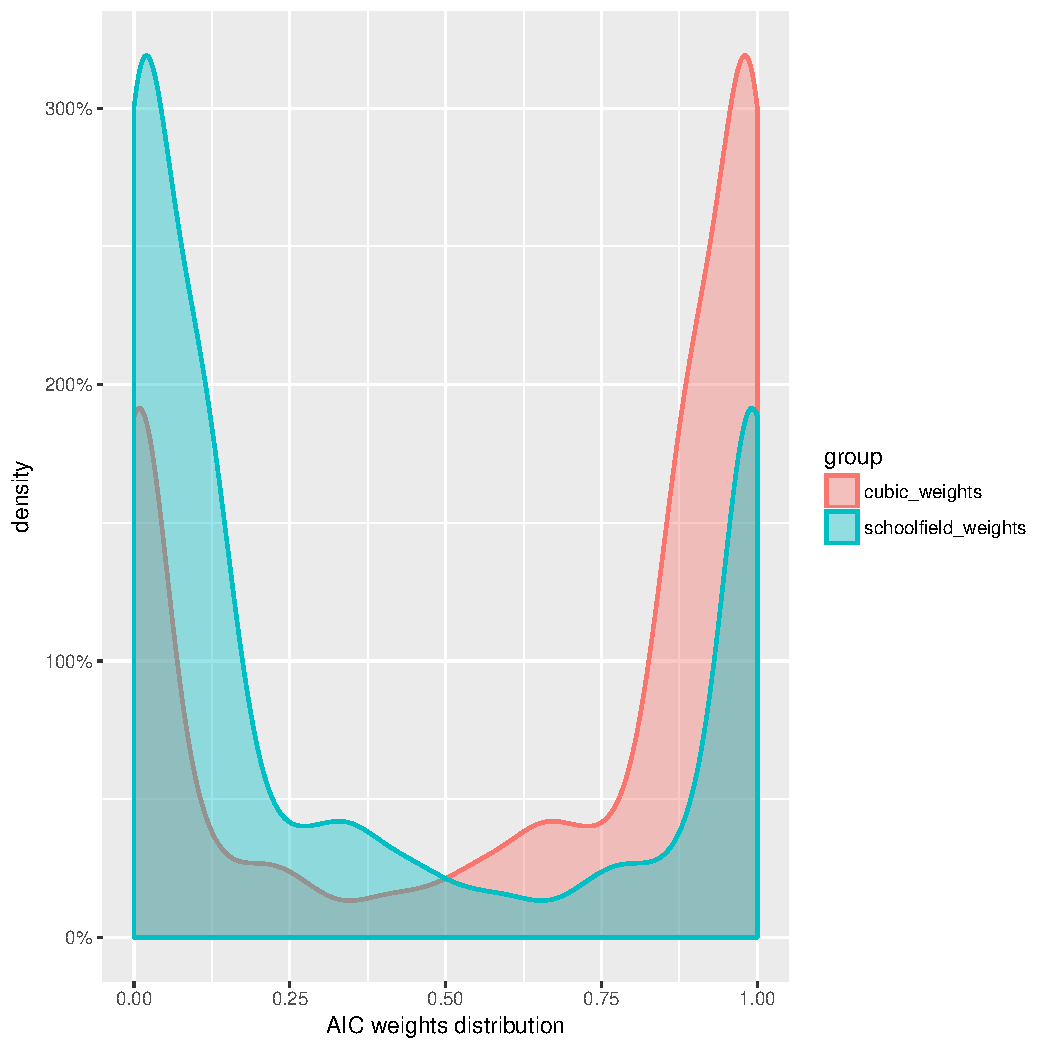
\includegraphics[width=0.7\textwidth]{../Results/general_plot.pdf}
	\caption{\label{fig:Akaike Weights}The distribution of Akaike Weights across the all traits for the cubic model and the Schoolfield model.}
\end{figure}

The Akaike weights, $W_i$, is a measure of certainty towards a model fitting the data and it is represented as a probability. The $W_i$ for the cubic model and Schoolfield model across all the traits were plotted and showed a general pattern of the cubic model having more best fits to the data compared to the Schoolfield model as seen in figure \ref{fig:Akaike Weights}. 

\begin{figure}[H]
	\centering
	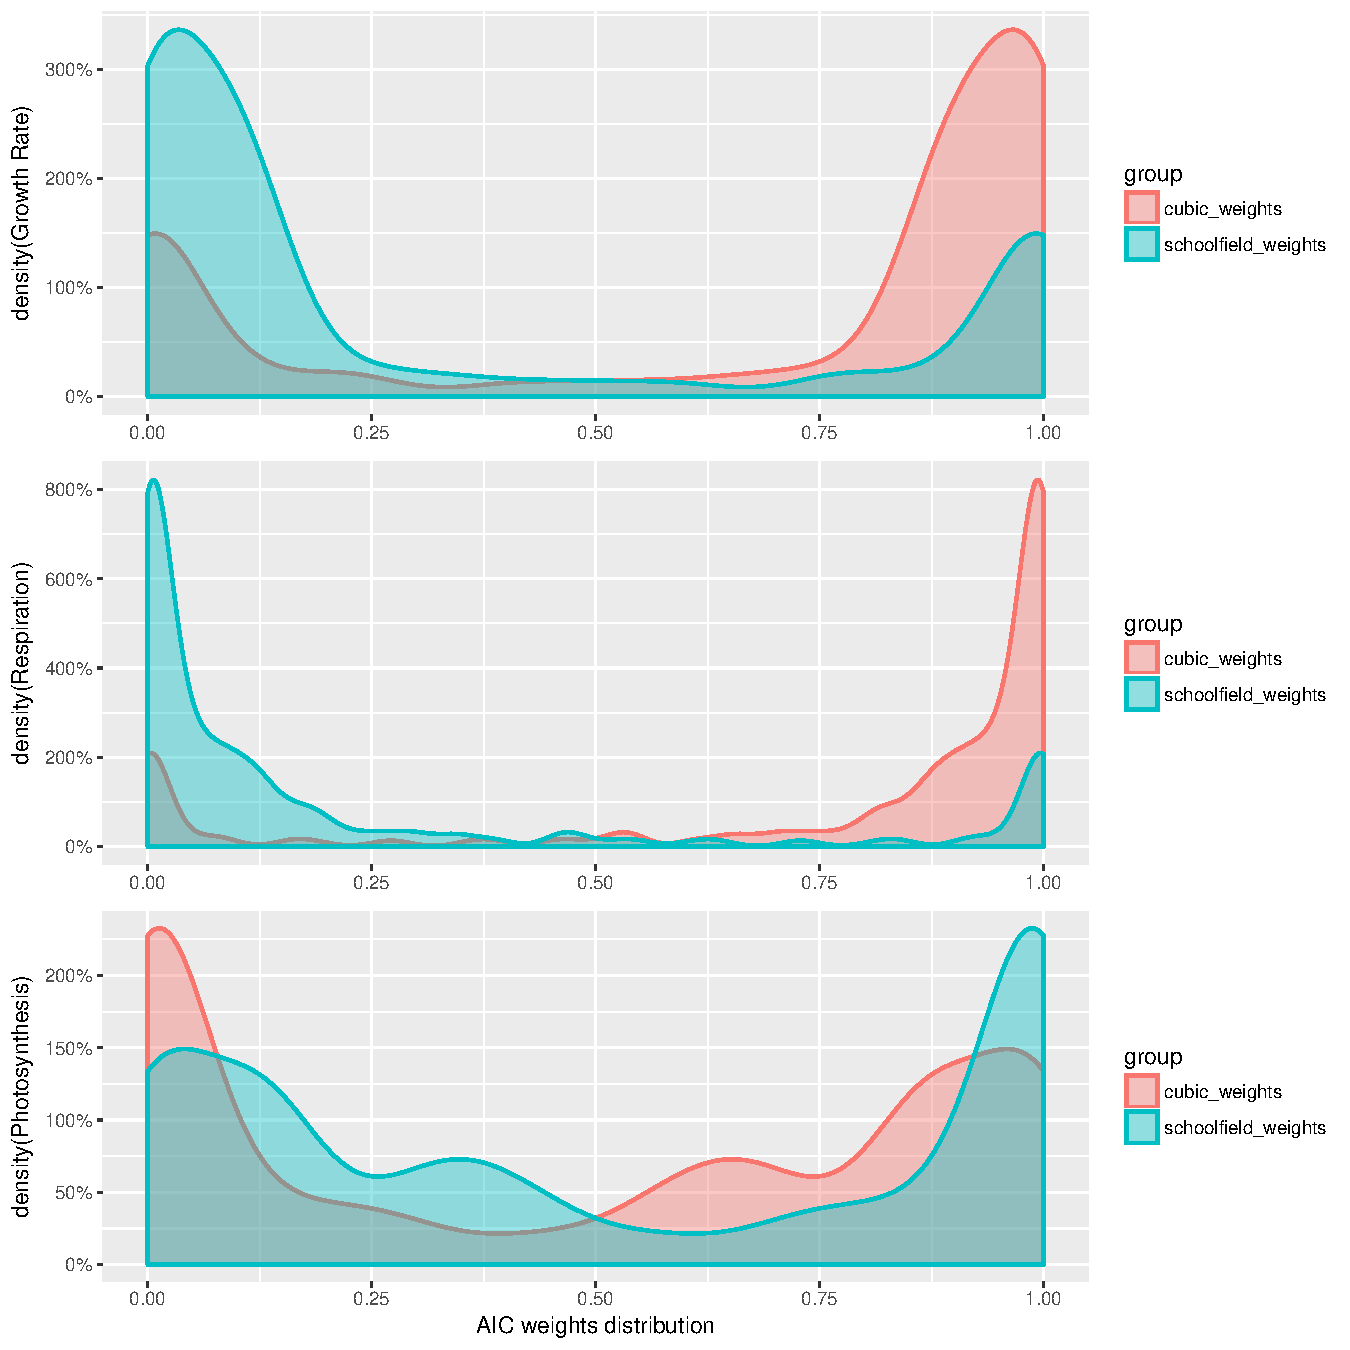
\includegraphics[width=.9\textwidth]{../Results/trait_plot.pdf}
	\caption{\label{fig:Akaike Weights by trait}The distribution of Akaike Weights across growth rate, respiration and photosynthesis traits for the cubic model and the Schoolfield model.}
\end{figure}

Figure \ref{fig:Akaike Weights by trait} shows the goodness of fit comparing both models for growth rate, photosynthesis and respiration. The plots showed that the cubic model had the higher likelihood as the best model for growth rate traits compared to the Schoolfield model, similarly the cubic model also a significantly better model for the respiration traits. However, the plot for the photosynthesis trait data represents a higher Akaike weights distribution for the Schoolfield model in contrast to the cubic model, suggesting that overall the Schoolfield model was the best model to describe photosynthesis traits. 

\section*{Discussion}

The NLLS fit produced a number of statistics such as chi-squared, r-squared, AIC and BIC results, from which only AIC and r-squared were extracted. AIC was chosen as one of the main statistical results to be analysed as it is good for cross referencing by calculating AIC $\Delta$ between models and does not penalise the number of parameters a model has. AIC does not make assumptions towards a true model existing in the dataset such as BIC does. BIC can give you a biased estimate if you have a small number of n data points measured \citep{Burnham2004}. Information drawn from AIC values are concise and easy to interpret and compare, however it is believed by some that inconsistencies occur with AIC because the AIC value for the model also reflects the quality of the data and therefore it can produce conflicting results \citep{Wagenmakers2004}. In addition, AIC does not take into account the differences in sampling range of the parameters estimated which can lead to inaccurate model selection results \citep{Wagenmakers2004}. 
\\~\\
Results from figure \ref{fig:NLLS_fit} shows that the Schoolfield model had the best fit to the data compared to the cubic model, this is reaffirmed by the statistical figures showing in Table 1 which shows a higher $chi^2$ and $R^2$ value, suggesting a Schoolfield having a better 'goodness of fit'. Moreover, the Schoolfield model has a lower AIC value in comparison to the cubic model and a $\Delta$ value of 0, this clearly suggests it is the best model out of the two to describe the data.
\\~\\
Despite results shown in fig \ref{fig:NLLS_fit}, the overall results as seen figure \ref{fig:Akaike Weights} show the cubic model having higher Akaike weightings across the whole dataset, this clearly suggest that the cubic model had a higher certainty that it fits the metabolic traits and thus it is the best model to describe the trait data. One reason the cubic model may have out performed the Schoolfield model is that it is a phenomenological model with unbounded parameters, whereas the Schoolfield model has mechanistic underpinnings and therefore has less flexibilitiy to fit its parameters to the data. Furthermore, the cubic model also has more degrees of freedom as it only has 4 parameters and when the models are being compared on the same number of data points, the cubic model has a more powerful ability to fit the data compared to the Schoolfied model which uses up more degrees of freedom as it has 6 parameters. 
\\~\\
In conclusion, although the cubic model is clearly seen to be the better model describing the data, there are other factors to consider such as the quality of the data and the reliability of statistical measurements.

\bibliographystyle{agsm}
\bibliography{Miniproject}

\end{document}